

%%%%%%%%%%%%%%%%%%%%%%%%%%%%%%%%%%%%%%%%%%%%%%%%%%%%%%%%%%%%%%%%%%%%%%

\begin{frame}[plain,label=Conc2]
\frametitle {Mass renormalisation on the threshold of Mott localisation}
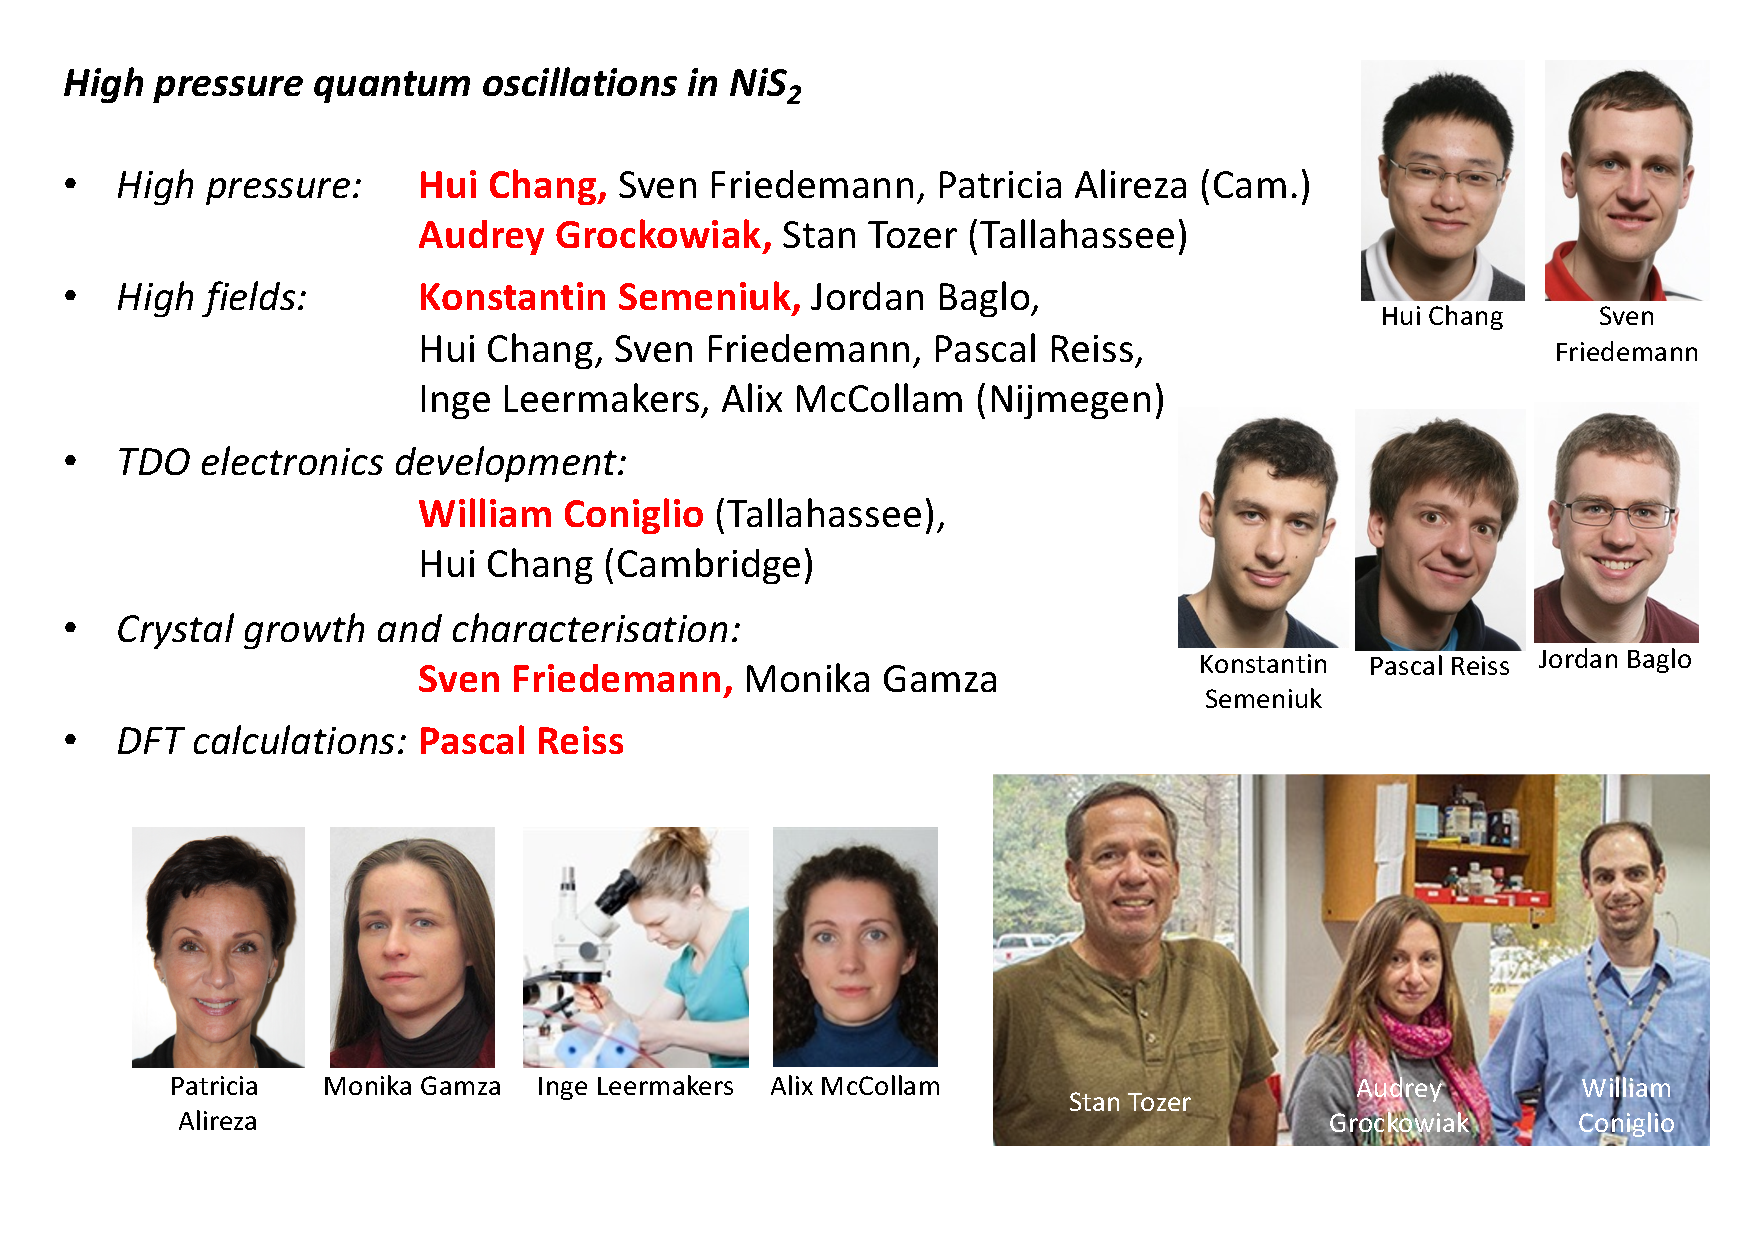
\includegraphics[width=1.2\textwidth]{GroupListNiS2}
\end{frame}

%%%%%%%%%%%%%%%%%%%%%%%%%%%%%%%%%%%%%%%%%%%%%%%%%%%%%%%%%%%%%%%%%%%%%%
\subsection{Mott Isolator NiS$_2$}
%%%%%%%%%%%%%%%%%%%%%%%%%%%%%%%%%%%%%%%%%%%%%%%%%%%%%%%%%%%%%%%%%%%%%%
\begin{frame}[label=NiS2-1]
\frametitle{Charge transfer Mott insulator Ni(S/Se)$_2$}
\begin{columns}[t]
\column{0.5\textwidth}
\centerline{~}
\centerline{\includegraphics[width=0.8\columnwidth]{\Figures/Structures/NiS2/NiS2.png}}

\begin{itemize}

\item
Descended from NiO
\item
fcc lattice of Ni in $d^8$ configuration.
\item
Charge gap between $3d$ UHB and S/Se $p$ states. 

\end{itemize}
\column{0.5\textwidth}
\centerline{~}
\centerline{\includegraphics[width=\columnwidth]{\data/NiS2/FiguresNiS2/BackgroundInfo/NiS2MiyasakaAnn}}
\end{columns}
\vspace{0.5em}
\centerline{Tuneable by isoelectronic Se doping or by pressure.}
\vspace*{\fill}
\vspace{-0.25em}
%\vspace{3.5em}
\centerline{\makebox[\linewidth]{\rule{0.85\textwidth}{0.4pt}}}
\centerline{\scriptsize Miyasaka et al, JPSJ {\bf 69,} 3166 (2000)}
\end{frame}





%%%%%%%%%%%%%%%%%%%%%%%%%%%%%%%%%%%%%%%%%%%%%%%%%%%%%%%%%%%%%%%%%%%%%%
%\subsection{High pressure NiS$_2$}
%%%%%%%%%%%%%%%%%%%%%%%%%%%%%%%%%%%%%%%%%%%%%%%%%%%%%%%%%%%%%%%%%%%%%%
\begin{frame}[label=NiS2-1]
\frametitle{Pressure induced Mott metal-insulator transition in NiS$_2$}
%\centerline{\includegraphics[width=\columnwidth]{\Figures/NiS2/PhaseDiaNiS2.pdf}}
\centerline{\includegraphics[width=0.8\columnwidth]{\data/NiS2/FiguresNiS2/Resistivity/SvenRes}}
\begin{itemize}
\item
Resistivity, liquid pressure medium, patterned anvils.

\item
Metallisation above 3 GPa in flux-grown high quality samples,
$\rho_0 < 1~\mu \Omega \mathrm {cm}$.

\item 
Search for quantum oscillations.

% \item
% AFM qcp at 8 GPa.
\end{itemize}
\vspace*{\fill}
\vspace{-0.25em}
%\vspace{3.5em}
\centerline{\makebox[\linewidth]{\rule{0.85\textwidth}{0.4pt}}}
\centerline{\scriptsize S. Friedemann Sci. Rep. {\bf 6,} 2535 (2016)}
\end{frame}

%%%%%%%%%%%%%%%%%%%%%%%%%%%%%%%%%%%%%%%%%%%%%%%%%%%%%%%%%%%%%%%%%%%%%
\subsection{High pressure QO}
%%%%%%%%%%%%%%%%%%%%%%%%%%%%%%%%%%%%%%%%%%%%%%%%%%%%%%%%%%%%%%%%%%%%%%
\begin{frame}[label=QuantOsc]
\frametitle{Quantum oscillations}
%\frametitle{Quantenoszillationen}

\visible<1->{\centerline{\includegraphics[width=0.8\columnwidth]{\Figures/Lectures/QuantOsc/Sr2RuO4Osc}}}


\visible<2->{
\centerline{\includegraphics[width=0.9\textwidth]{\Figures/FermInstab/QuantOsc-Xray.pdf}}}

\end{frame}

%%%%%%%%%%%%%%%%%%%%%%%%%%%%%%%%%%%%%%%%%%%%%%%%%%%%%%%%%%%%%%%%%%%%%%
%\subsection{rf methods}
%%%%%%%%%%%%%%%%%%%%%%%%%%%%%%%%%%%%%%%%%%%%%%%%%%%%%%%%%%%%%%%%%%%%%%
%%%%%%%%%%%%%%%%%%%%%%%%%%%%%%%%%%%%%%%%%%%%%%%%%%%%%%%%%%%%%%%%%%%%%%
\begin{frame}[label=DACcoil]
\frametitle{Quantum oscillation measurements at high pressure}

\centerline{\includegraphics[width=0.9\columnwidth]{\Figures/Pressure/TDO/QO-DAC-TDO}}
\begin{itemize}

\item
%Developed for magnetic susceptibility measurements, 
Coil in sample space, filling factor $\sim 0.3$

\item
At high frequency, probe metallic skin depth $s \propto
\sqrt{\rho/\omega}$.

\item 
Skin depth $\rightarrow$ excluded sample volume $\rightarrow$ \\ \raggedleft{coil
self-inductance $\rightarrow$ resonance frequency.}
% Resolution $\delta L/L \simeq f \frac{s}{r} \delta \rho/\rho$.\\ {\small ($f =$ coil filling factor, $r = $ sample radius)} 
\end{itemize}


\vspace*{\fill}
%\vspace{3.5em}
\centerline{\makebox[\linewidth]{\rule{0.85\textwidth}{0.4pt}}}
\centerline{\scriptsize Alireza, Rev. Sci. Inst. {\bf 74,} 4728 (2003)}

\end{frame}


%%%%%%%%%%%%%%%%%%%%%%%%%%%%%%%%%%%%%%%%%%%%%%%%%%%%%%%%%%%%%%%%%%%%%
%\section{NiS$_2$ Quantum oscillations}
%%%%%%%%%%%%%%%%%%%%%%%%%%%%%%%%%%%%%%%%%%%%%%%%%%%%%%%%%%%%%%%%%%%%%
\begin{frame}[label=NiS2Mass]
  \frametitle{Fermi surface and effective mass in pressure metallised NiS$_2$}
\centerline{\includegraphics[width=\columnwidth]{\data/NiS2/FiguresNiS2/HomeDetail/QOPlot3FigText}}
%
%\begin{itemize}
%\item Amplitude boosted compared to lower pressure measurement.
%\item 6 kT frequency $\rightarrow$ large hole pocket as in DFT calculation. 
%
%\item Mass $\simeq 5\times$ band mass.
%%\item Amplitude much higher than at lower $p$ near Mott transition:
% %  phase coexistence at low $p$?
%\end{itemize}


\vspace*{\fill}
\centerline{\makebox[\linewidth]{\rule{0.85\textwidth}{0.4pt}}}
\begin{center}
{\scriptsize K. Semeniuk, H. Chang, J. Baglo, S. Friedemann, A. Grockowiak, \\
A. McCollam et al (Nijmegen/Tallahassee/Cambridge),  \hlb{arXiv: 2202.04024 (2022)}}
\end{center}

\end{frame}





%%%%%%%%%%%%%%%%%%%%%%%%%%%%%%%%%%%%%%%%%%%%%%%%%%%%%%%%%%%%%%%%%%%%%
%\subsection{Mass and frequency vs. $p$}
% %%%%%%%%%%%%%%%%%%%%%%%%%%%%%%%%%%%%%%%%%%%%%%%%%%%%%%%%%%%%%%%%%%%%%
\begin{frame}[label=QONiS2]
\frametitle{Evolution of Fermi surface and effective mass in NiS$_2$}
\vspace{0.5em}

\centerline{\includegraphics[width=0.9\columnwidth]{\data/NiS2/FiguresNiS2/PressureDependence/Fig3_PressureDep4FignoLabels}}
\begin{itemize}
\item
Fermi surface stays large on approaching Mott transition, but
effective mass rises.
\item
Divergence \hl{inside} insulating region.
\end{itemize}

\vspace*{\fill}
\centerline{\makebox[\linewidth]{\rule{0.85\textwidth}{0.4pt}}}
\begin{center}
{\scriptsize K. Semeniuk, H. Chang, J. Baglo, S. Friedemann, A. Grockowiak, \\
A. McCollam et al (Nijmegen/Tallahassee/Cambridge),  \hlb{arXiv: 2202.04024 (2022)}}
\end{center}

\end{frame}


